
\subsection{Conexo no implica arco conexo}
Sea $S = \{(t, \sin \frac 1t): t geq 0\} \subseteq \mathbb R^2$ curva del topologo que cumple:

\begin{itemize}
    \item S es arco conexo,
    \item Luego S es conexo, $\overline S$ es conexo. (Teorema de clase )
\end{itemize}

\paragraph{Lemma:} $\overline S$ no es arco conexo.



\begin{center}
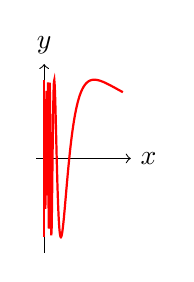
\begin{tikzpicture}[scale=1]
  % Axes
  \draw[->] (-0.1,0) -- (1.1,0) node[right] {$x$};
  \draw[->] (0,-1.2) -- (0,1.2) node[above] {$y$};
  % Graph of sin(1/x) for x>0
  \draw[red, thick, domain=0.015:1, samples=200] plot (\x,{sin(deg(1/\x))});
  % Closure segment at x=0
  \draw[red, thick] (0,-1) -- (0,1);
\end{tikzpicture}
\end{center}


\paragraph{Demostración:} Queremos mostrar que $(0,0)$ no se conecta con camino a ningún punto de $S$

Supongamos que $\gamma: [0,1] \to \overline S$ es un camino con $\gamma(0) = (0,0)$ y $\gamma(1) \in S$. En algún momento el camino tendrá que salir. Asi definimos:

\begin{align*}
    A = \{t \in [0,1]: \gamma(t) \in \{0\} \times [-1,1]\} \\
\end{align*}

Satisface que:

\begin{itemize}
    \item $A \neq \emptyset$ porque $(0,0) \in A$.
    \item $A$ es cerrado, $A = f^{-1}(\{0\}) \times [-1,1]$ con $\{0\} \times [-1,1] \overset{\text{cerr}}\subseteq \mathbb R^2$.
        \item $A$ es acotado superiormente, $1$ es cota superior. Luego $A$ tiene un elemento máximo digamos $a$. El supremo se vuelve un máximo pues $A$ es cerrado. Asi $a<1$
        \begin{align*}
            \gamma: [0,1] &\to \overline S \\
        \end{align*}

        Consideremos $\gamma|_{(a,1]}$:


        
        \begin{center}
            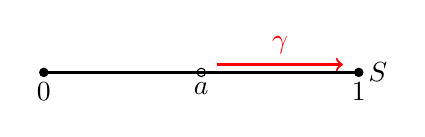
\begin{tikzpicture}[scale=1]
            % Interval illustration: points 0, a, 1 and mapping γ to S
            \draw[thick] (0,0) -- (4,0);
            \draw[fill] (0,0) circle (1.5pt) node[below] {$0$};
            \draw (2,0) circle (1.5pt) node[below] {$a$};
            \draw[fill] (4,0) circle (1.5pt) node[below] {$1$};
            \draw[->, red, thick] (2.2,0.1) -- (3.8,0.1) node[midway, above] {$\gamma$};
            \node[right] at (4,0) {$S$};
            \end{tikzpicture}
        \end{center}



        Para $t\in (a,1]$, $\gamma(t) = \left(x(t),\sin \left(\frac{1}{x(t)}\right) \right)$. Tomemos  $x_n = \frac{1}{n\pi}$, para $n$ suficientemente grande (punto azules). Observemos que:

        \begin{center}
            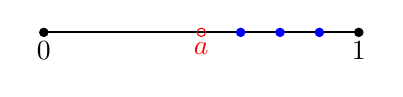
\begin{tikzpicture}[scale=1]
              % Interval with sequence points x_n between a and 1
              \draw[thick] (0,0) -- (4,0);
              \draw[fill] (0,0) circle (1.5pt) node[below] {$0$};
              \draw[red] (2,0) circle (1.5pt) node[below] {$a$};
              % Sequence points (blue) approaching from the right
              \draw[fill,blue] (2.5,0) circle (1.5pt);
              \draw[fill,blue] (3.0,0) circle (1.5pt);
              \draw[fill,blue] (3.5,0) circle (1.5pt);
              \draw[fill] (4,0) circle (1.5pt) node[below] {$1$};
            \end{tikzpicture}
        \end{center}



        \begin{align*}
            \sin \left(\frac{1}{x_n}\right) &= \sin(n\pi) = (-1)^n \\
        \end{align*}

        \begin{center}
            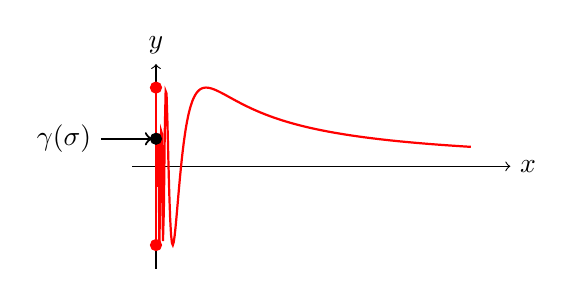
\begin{tikzpicture}[scale=1]
              % Coordinate axes
              \draw[->] (-0.3,0) -- (4.5,0) node[right] {$x$};
              \draw[->] (0,-1.3) -- (0,1.3) node[above] {$y$};
            
              % Graph of  sin(1/x) for x > 0
              \draw[red, thick, domain=0.02:4, samples=350] plot (\x,{sin(deg(1/\x))});
            
              % Closure segment at x = 0
              \draw[red, thick] (0,-1) -- (0,1);
            
              % End‑points of the closure segment
              \foreach \y in {-1,1}{
                \draw[fill,red] (0,\y) circle (2pt);
              }
            
              % A point γ(σ) on the segment and its label
              \draw[fill] (0,0.35) circle (2pt);
              \draw[->, thick] (-0.7,0.35) -- (-0.05,0.35);
              \node[left] at (-0.7,0.35) {$\gamma(\sigma)$};
            \end{tikzpicture}
        \end{center}

        Restringimos la curva a una $\alpha: (0,1] \to S$, talque:

        \begin{align*}
            \alpha(t) &= \gamma( a+t(1-a)) \\
        \end{align*}

        $\alpha$ es continua, $x_n \to 0$, $n \to \infty$, y como $\alpha$ es continua, $\alpha \left(\frac{1}{\pi n},(-1)^n\right)=\alpha(x_n) \to \alpha(0) = \gamma(a) \in \{0\} \times [-1,1]$. Luego:
        \begin{align*}
            \left(\frac 1{\pi n}, (-1)^n\right) \text{ converge }
        \end{align*}

        y por lo tanto $(-1)^n$ converge, lo cual no lleva a una contradicción, pues $(-1)^n$ no converge. 
        La contradicción esta en suponer que $\overline S$ es arco conexo. Y por lo tanto:
        % pues en otro caso $\gamma(1) \notin S$. Consideremos la sucesion $\left\{a+\frac 1n\right\}_{n>N}$, tal que $a<a+\frac 1n<1$, tenemos que $\gamma(a+\frac 1n) \in S$ y $\gamma(a+\frac 1n) = (a_n, \sin \frac 1{a_n})$. Como $\gamma$ es continua, $\gamma(a+\frac 1n) \to \gamma(a) = (0,0)$, $\gamma(a) \in \{0\} \times [-1,1]$, pues como $\gamma$ es continua, debe enviar sucesiones convergentes a sucesiones convergentes. Asi:
        % \begin{align*}
        %     \left(a_n, \sin \frac 1{a_n}\right) &\to (0,0) 
        %                     n&\to \infty \\
        % \end{align*}
        % luego $x_n \to 0$, $\sin \left(\frac 1{x_n}\right) \to 0$. Esto es imposible porque $f(x) = \sin \frac 1x$ no es continua en 
\end{itemize}


\paragraph{Observacion:} Conexo no implica arco conexo.
\paragraph{Nota:}La clase anterior se demostró que arco conexo implica conexo.

\paragraph{Ejercicios:}
\begin{enumerate}
    \item  Imagen de conexo (arco conexo) bajo una función continua es conexo (arco conexo).
    \item Demostrar que $A\subseteq \mathbb R$ es conexo si y solo si $A$ es un intervalo.
\end{enumerate}

\paragraph{Nota:} $A$ es un intervalo si para todo $a,b \in A$, $(a,b) \subseteq A$.

\paragraph{Teorema:} Si $A \overset{\text{ab}}\subseteq \mathbb R^n$ tal que $A$ es conexo, entonces $A$ es arco conexo.

\paragraph{Demostración:} 
\begin{center}
\noindent\fbox{%
\parbox{0.95\textwidth}{%
\paragraph{Lema:} $A$ es conexo si y solo si los únicos abierto y cerrados son $A$ y $\emptyset$.%
}}
\end{center}

Sea $x_0 \in A$ , consideremos el conjunto $B\in \{x \in A: \exists \gamma: [0,1]\to A \text{ continua, } \gamma(0) = x_0 \land \gamma(1)=x\}$, es decir $x_0$ y $x$ se conectan por un camino.
\begin{center}
    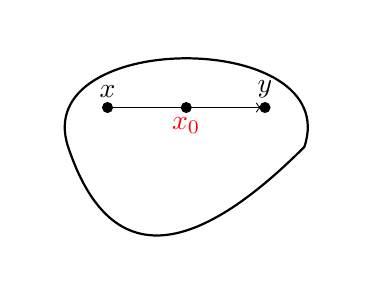
\begin{tikzpicture}[scale=1]
      % Enclosing blob
      \draw[thick] (-1.5,-0.5) .. controls (-2,1) and (2,1) .. (1.5,-0.5) .. controls (0,-2) and (-1,-2) .. cycle;
      % Points x, x0, y
      \fill (-1,0) circle (2pt) node[above] {$x$};
      \fill (0,0) circle (2pt) node[below, red] {$x_0$};
      \fill (1,0) circle (2pt) node[above] {$y$};
      % Arrows between points
      \draw[->] (-1,0) -- (0.05,0);
      \draw[->] (0,0) -- (0.95,0);
    \end{tikzpicture}
\end{center}


Veamos que $B$ es abierto y cerrado. Veamos $x_0 \in B$, pues $x_0$ se conecta a si mismo por el camino constante. Queremos ver que $B= A$

\begin{itemize}
    \item $B$ es abierto, sea $x\in B$m existe una vecindad abierta $U$ de $x$, $U$ es arco conexo y $x \in U$, queremos ver que $U\subseteq B$. 

    \begin{center}
    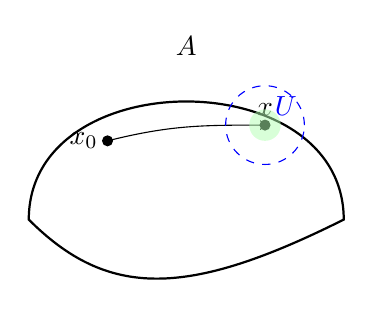
\begin{tikzpicture}[scale=1]
      % Enclosing set A
      \draw[thick] (-2,-1) .. controls (-2,1) and (2,1) .. (2,-1) .. controls (0,-2) and (-1,-2) .. cycle;
      \node at (0,1.2) {$A$};
      % Point x_0 and arrow to x
      \fill (-1,0) circle (2pt) node[left] {$x_0$};
      \draw[->] (-1,0) .. controls (-0.2,0.2) and (0.2,0.2) .. (1,0.2);
      \fill (1,0.2) circle (2pt) node[above] {$x$};
      % Open neighborhood U around x
      \draw[dashed, blue] (1,0.2) circle (0.5) node[above right] {$U$};
      % Small filled region inside U
      \fill[green!30, opacity=0.5] (1,0.2) circle (0.2);
    \end{tikzpicture}
    \end{center}


    Sea $\gamma_1$ un camino de $x_0$ a $x$, sea $y \in U$, como $U$ es arco conexo, existe un camino $\gamma_2$ de $x$ a $y$, entonces la concatenación $\gamma_1 * \gamma_2$ es un camino que conecta $x_0$ con $y$, luego $y \in B$ y entonces $U \overset{\text{ab}}\subseteq A$.

   
    \item $B$ es cerrado, $x \in A-B$, no existe un camino de $x_0$ a $x$.
    Un argumento similar al anterior, demuestra que existe una vecindad abierta $U$ de $x$ tal que $U \cap A/B$, luego $A-B$ es abierto en $A$, es decir $B$ es cerrado. Como $A$ es conexo, y $B \neq \emptyset$, $B = A$, es decir, todo elemento se conecta a $x_0$ y por lo tanto $A$ es arco conexo.

    \begin{center}
        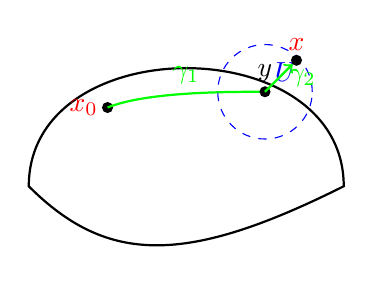
\begin{tikzpicture}[scale=1]
          % Conjunto A
          \draw[thick] (-2,-1) .. controls (-2,1) and (2,1) .. (2,-1) .. controls (0,-2) and (-1,-2) .. cycle;
          % Punto x_0 y trayectoria gamma1
          \fill (-1,0) circle (2pt) node[left, red] {$x_0$};
          \draw[green, thick] (-1,0) .. controls (-0.5,0.2) and (0.5,0.2) .. (1,0.2) node[midway, above] {$\gamma_1$};
          % Punto y
          \fill (1,0.2) circle (2pt) node[above] {$y$};
          % Vecindad U alrededor de y
          \draw[dashed, blue] (1,0.2) circle (0.6) node[above right] {$U$};
          % Punto x y trayectoria gamma2
          \fill (1.4,0.6) circle (2pt) node[above, red] {$x$};
          \draw[->, green, thick] (1,0.2) -- (1.35,0.55) node[midway, right] {$\gamma_2$};
        \end{tikzpicture}
        \end{center}

    \hfill $\square$
\end{itemize}

\paragraph{Ejercicio} En $\mathbb R^n$ la bolas abiertas son arco conexas.


\subsection{Puntos de corte}

\paragraph{Definición:} Sea $X$ conexo, un punto de corte $x \in X$ es tal que $X - \{x\}$ es disconexo. 

\paragraph{Observación:} Si $f: X \to Y$ homeomorfismo, entonces si $x$ es punto de corte de $X$, $f(x)$ es punto de corte de $Y$.
\paragraph{Demostración:} Ejercicio.
\paragraph{Ejemplos:}
\begin{itemize}
    \item Es $\mathbb R \simeq \mathbb R^2$ ?  No porque por ejemplo $x\in \mathbb R$ es punto de corte, mientra que en $\mathbb R^2$ no hay puntos de corte.
    \begin{center}
        \begin{tikzpicture}[scale=1]
          % Coordinate axes
          \draw[->] (-2,0) -- (2,0) node[right] {$x$};
          \draw[->] (0,-2) -- (0,2) node[above] {$y$};
          % Origin highlight
          \draw[fill] (0,0) circle (2pt) node[below right] {$0$};
          % Points and path around origin
          \fill (-1,0.5) circle (2pt) node[left] {};
          \fill (1,1.5) circle (2pt) node[right] {};
          \draw[thick, red, ->] (-1,0.5) .. controls (0.5,0.5) and (0.5,1.5) .. (1,1.5);
        \end{tikzpicture}
    \end{center}

    \item La siguientes figuras:

    \begin{center}
        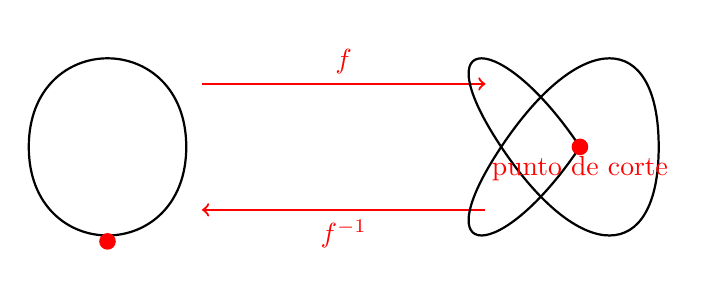
\begin{tikzpicture}[scale=1]
          % Bucle simple (sin puntos de corte) con punto marcado
          \draw[thick] (-3,0) .. controls (-3,1.5) and (-1,1.5) .. (-1,0)
                         .. controls (-1,-1.5) and (-3,-1.5) .. cycle;
          \fill[red] (-2,-1.2) circle (3pt) node[below] {};
        
          % Flechas f y f^{-1}
          \draw[->, red, thick] (-0.8,0.8) -- (2.8,0.8) node[midway, above] {$f$};
          \draw[->, red, thick] (2.8,-0.8) -- (-0.8,-0.8) node[midway, below] {$f^{-1}$};
        
          % Figura en ocho con punto de corte
          \draw[thick] (3,0) .. controls (2,1.5) and (3,1.5) .. (4,0)
                         .. controls (3,-1.5) and (2,-1.5) .. cycle;
          \draw[thick] (3,0) .. controls (4,1.5) and (5,1.5) .. (5,0)
                         .. controls (5,-1.5) and (4,-1.5) .. cycle;
          \fill[red] (4,0) circle (3pt) node[below] {punto de corte};
        \end{tikzpicture}
    \end{center}
    
    \item $S^1 \not \simeq \mathbb R$ pues $S^1$ no tiene puntos de corte, mientras que $\mathbb R$ tiene infinitos puntos de corte.
\end{itemize}

\subsection{Componentes conexas y arco conexas}
\paragraph{Definición:} Sea $X$ un espacio topológico, una componente conexa(arco conexa) es un subespacio $Y \subseteq X$ tal que $Y$ es conexo (arco conexo) y talque $Z \subseteq X$ es conexo(arco conexo) y $Y \subseteq Z$ implica que $Y = Z$. (Maximal conexo), la definición de componente arco conexa es similar.

\paragraph{Observaciónes:} 
\begin{itemize}
    \item $X$ se expresa como union disyunta de sus componentes conexas(arco conexas)
    \item Dos componentes conexas son disjuntas. Sale por definición.
    \item Todo elemento esta contenido en una componente conexa.
    Dado $x \in X$, consideramos $\mathcal f = \{C \subseteq X: C \text{ conexo y } x \in C\}$, $\bigcup \mathcal f$ es conexo, por que es union de conexos con un punto en común. Notemos que la familia $\mathcal f$ es no vacía por los singletons. Ademas $\bigcup \mathcal f$ es maximal, luego $\bigcup \mathcal f$ es una componente. Para arco conexidad es similar.
    \item Dado $x \in X$, la componente arco conexa que contiene a $x$ es el conjunto:
    \begin{align*}
        P(x) = \{y \in X: x \land y \text{ se conectan por un camino}\}
    \end{align*}
    Cumple las siguientes propiedades:
    \begin{itemize}
        \item $P(x)$ es arco conexo.
        \item $P(x)$ es arco conexo maximal, luego $P(x)$ es la componente arco conexa que contiene a $x$.
    \end{itemize}
\end{itemize}.

\paragraph{Proposición:} Si todo punto de un espacio topológico $X$ tiene una vecindad arco conexa, entonces las vecindades arco conexas de $X$ son tambien las componentes conexas. (Ejercicio)


\paragraph{Nota muy importante:} Hasta aquí tenemos el quiz.


\paragraph{Ejercicios:} 
\begin{itemize}
    \item Hatcher pg 25
    \begin{itemize}
        \item $3 - 6$
    \end{itemize}
    \item Viro - Ivanov. Pg 45
    \begin{itemize}
        \item 9.U 
        \item 10.1
        \item 10.7
        \item 10.P 
        \item 10.19
        \item 10.20
    \end{itemize}
\end{itemize}

